\documentclass{article}
\usepackage{graphicx}
\usepackage{tikz}

\title{Probability and Randomization}
\author{Course Staff}

\begin{document}
\maketitle

\section{Probability rules}

For an event $A$, the complement rule is
\[
  \Pr(A^{\mathsf c}) = 1 - \Pr(A).
\]

\begin{table}
  \centering
  \caption{A simple probability distribution}
  \begin{tabular}{lr}
    Outcome & Probability \\
    Control & 0.50 \\
    Treatment & 0.50
  \end{tabular}
\end{table}

\begin{figure}
  \centering
  % allytex: alt=Two study arms branch from one randomized cohort.
  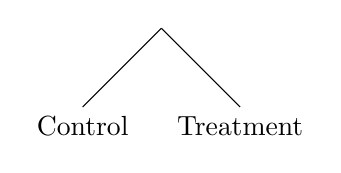
\begin{tikzpicture}
    \draw (0,0) -- (-1,-1) node[below] {Control};
    \draw (0,0) -- (1,-1) node[below] {Treatment};
  \end{tikzpicture}
  \caption{Randomization into two study arms}
\end{figure}


\begin{tikzpicture}
  \node[draw] {Generated placeholder test};
\end{tikzpicture}

\setlength{\unitlength}{1pt}
\begin{picture}(30,12)
  \put(0,1){\line(1,0){30}}
\end{picture}

Inline drawing: \tikz[baseline]{\draw (0,0) -- (0.5,0);}

\end{document}
